\subsection{Within-Database Experiments}
\subsubsection{Finger Knuckle V3 Database with Deformation}

The Finger Knuckle V3 Database have 1-104 subjects that have two session samples, and the rest subjects of first session 105-221 just offer one session samples. So as the first experiment, I firstly fine-tuned my model on the second session of 1-104 subjects, and test on the first session 1-104 subjects. So it will have $104*6=624$ genuine matching scores, and have $104*103*6=64272$ imposter matching scores. From the below figure, if the false accept rate is below $10^{-2}$, the RFN-128-WRS is better than the RFN-128-WS. I also use the FKNet to train on this database, and the performance of FKNet is not better than the RFNet depend on the ROC figure. From the CMC and ROC, each model with WRS is better than WS on this dataset. \textcolor{red}{For the ROC curve, I add EfficientNetV2-S model performance.}

\begin{figure}[H]
	\centering
	\begin{subfigure}[b]{0.8\linewidth}
		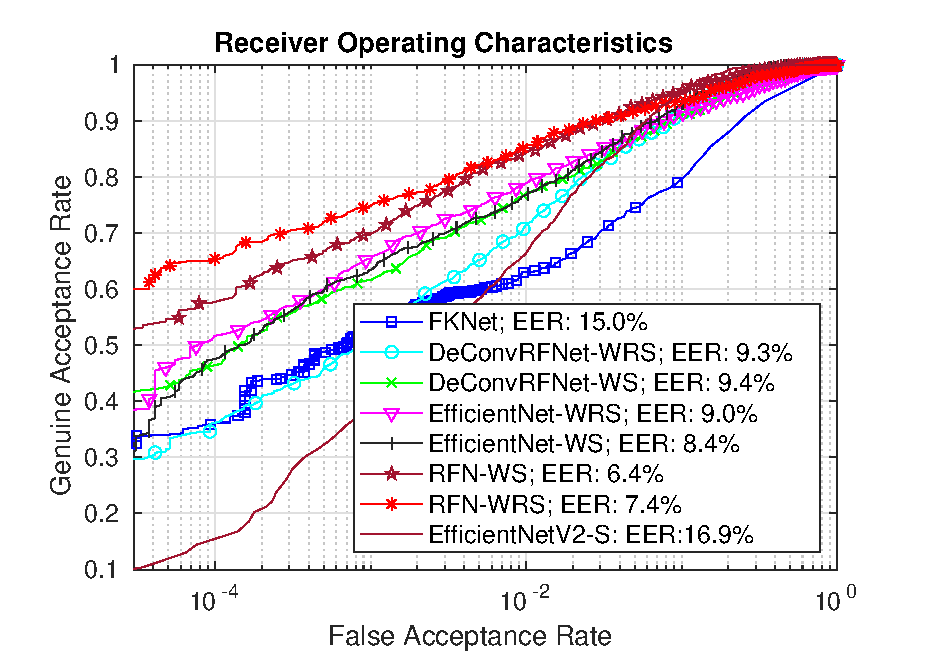
\includegraphics[width=\linewidth]{Figures/add-efficientv2-s/fkv3-roc_compare_new.eps}
	\end{subfigure}
	\begin{subfigure}[b]{0.8\linewidth}
		\includegraphics[width=\linewidth]{Figures/fknet/fkv3-cmc.eps}
	\end{subfigure}
\end{figure}



As for the two-session protocol on the database. I should fine-tune my model on the 105-221 subjects, and use two-session protocol to evaluate my model performance on the 1-104 subjects dataset. In totally, it will generate $104*6=624$ genuine scores, and $104*103*6$ imposter scores. However, the FKNet is a classification task, and the output number classes should be same when training and testing. So the two session protocol experiment is not fit for FKNet. If the FKNet train on the 105-221 subjects and test on the 1-104 subjects with two sessions, the classes is different.

\begin{figure}[H]
    \centering
    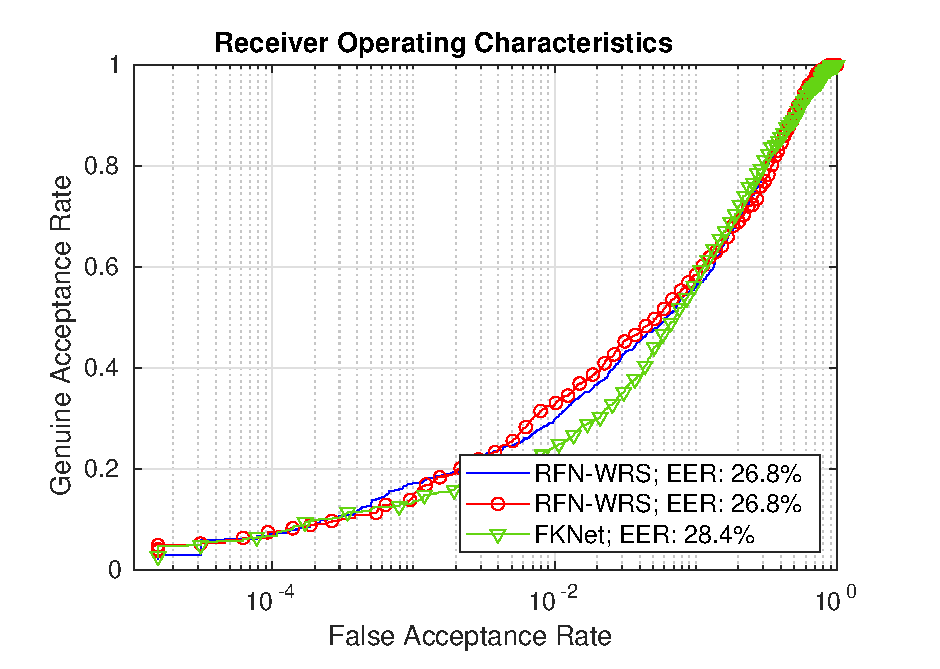
\includegraphics[width=0.8\linewidth]{Figures/fknet/two-fkv3-roc_compare_new.eps}
\end{figure}

The two-session protocol will use the session1 as the probe and use the session2 as the enrollment. As for the genuine matching scores, each sample of a subject will choose the minimal matching score when compare to the rest samples. In this kind of situation, it will have $104x6$ genuine matching scores. Meanwhile, as for the imposter matching scores, it will also choose the minimal value result in $104*103*6$ imposter matching scores on the confusion matrix.